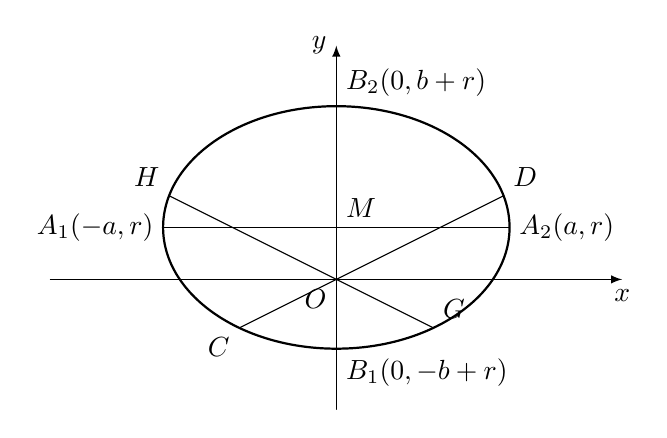
\begin{tikzpicture}[>=latex, scale=1.1, line join=round, line cap=round]
  % Axes
  \draw[->] (-3.3, 0) -- (3.3, 0) node[below] {$x$};
  \draw[->] (0, -1.5) -- (0, 2.7) node[left] {$y$};
  \node[below left] at (0, 0) {$O$};

  % Center M and major axis A1A2
  \coordinate (M) at (0, 0.6);
  \node[above right] at (M) {$M$};
  \coordinate (A1) at (-2.0, 0.6);
  \coordinate (A2) at (2.0, 0.6);
  \draw (A1) -- (A2);
  \node[left] at (A1) {$A_1(-a,r)$};
  \node[right] at (A2) {$A_2(a,r)$};

  % Ellipse
  \draw[thick] (M) ellipse (2.0 and 1.4);

  % Vertices on y-axis
  \node[above right] at (0, 2.0) {$B_2(0, b+r)$};
  \node[below right] at (0, -0.8) {$B_1(0, -b+r)$};

  % Intersections of lines y = k1 x and y = k2 x
  \coordinate (D) at (1.93, 0.965);
  \coordinate (C) at (-1.12, -0.56);
  \coordinate (H) at (-1.93, 0.965);
  \coordinate (G) at (1.12, -0.56);

  \draw (C) -- (D);
  \draw (H) -- (G);

  \node[above right] at (D) {$D$};
  \node[below left] at (C) {$C$};
  \node[above left] at (H) {$H$};
  \node[above right] at (G) {$G$};
\end{tikzpicture}
